\documentclass[10pt]{beamer}
% \documentclass[handout,10pt]{beamer}
\usepackage{my_style}

\title[Math/CS 375]{Lecture 15 - C}
\subtitle{\S 7.1, 7.2, 7.3 Runge-Kutta Methods}

\begin{document}
% -------------------------------------------------
\begin{frame}
  \titlepage
\end{frame}
% -------------------------------------------------
\begin{frame}{Goals}
We will answer these questions:\\[3mm]
\begin{itemize}
    
    \item What is the main idea behind the Runge-Kutta methods?

    \item How are the RK2 methods derived?
    
    \item How does classical RK4 combine four slope evaluations?
    
    \item How do the RK2 and RK4 methods compare to Euler's method in terms of accuracy? 
    
    \item How do we choose the step size for Runge-Kutta methods?
\end{itemize}
\end{frame}




%%%%%%%%%%%%%%%%%%%%%%%%%%%%%%%%%%%%%%
\sectionframe{Runge-Kutta Methods}
%%%%%%%%%%%%%%%%%%%%%%%%%%%%%%%%%%%%%%
\begin{frame}{Fundamental Theorem}
\begin{itemize}
    \item The goal is to solve the ODE 
    $$
    u'=f(t,u) 
    $$
    \item We can use the fundamental theorem 
    \begin{align*}        
    \int_{t_i}^{t_{i+1}} u' \,dt &= \int_{t_i}^{t_{i+1}} f(t,u) \,dt\\
     u(t_{i+1})-u(t_i)  &= \int_{t_i}^{t_{i+1}} f(t,u) \,dt\\
     u(t_{i+1})  &= u(t_i)+\int_{t_i}^{t_{i+1}} f(t,u) \,dt
    \end{align*}

    \begin{block}{Heart of Runge-Kutta Methods}
        $$
             u(t_{i+1})  = u(t_i)+\int_{t_i}^{t_{i+1}} f(t,u) \,dt
        $$
    \end{block}
\end{itemize}
\end{frame}

% --------------------------

\begin{frame}{Runge-Kutta Time Stepping}
    \begin{itemize}
        \item \textbf{Runge-Kutta} methods are derived by approximating the integral in 
            $$
            u(t_{i+1}) = u(t_i) + \underbrace{\int_{t_i}^{t_{i+1}} f(t, u(t)) \, dt}_{\text{approximate}}
            $$
        and developing a time-stepping algorithm\\[3mm]

    \end{itemize}
    \method{Runge-Kutta}{Initial Value Problem, time discretization $h$}{Discrete solution $\textbf{u}$}{Approximate $\int_{t_i}^{t_{i+1}} f(t, u(t)) \, dt$ with a quadrature}
\end{frame}
% --------------------------

\begin{frame}{Euler's Method}

\begin{itemize}

    \item Consider the simple Riemann approximation
    $$
        \int_a^b f(x)\,dx \approx (b-a) f(a)
    $$

    \item Apply this approximation  
    \begin{align*}        
     u(t_{i+1})  &= u(t_i)+\int_{t_i}^{t_{i+1}} f(t,u) \,dt\\
       u(t_{i+1}) &\approx  u(t_i)+(t_{i+1}-t_i) f(t_i,u(t_i))\\
    u_{i+1} &=  u_i+h\;f(t_i,u_i)
    \end{align*}
    \item The result is \textit{Euler's method}

    \keyidea{Euler's method can be thought of as a low-order Runge-Kutta method.}
\end{itemize}
\end{frame}
%%%%%%%%%%%%%%%%%%%%%%%%%%%%%%%%%%%%%%%%%%%%

\begin{frame}{Better Quadratures}

\question{What happens when you apply better quadratures to 
            $$
            u(t_{i+1}) = u(t_i) + \underbrace{\int_{t_i}^{t_{i+1}} f(t, u(t)) \, dt}_{\text{approximate}}\;?
            $$
            }

\begin{itemize}
    \item Trapezoid Rule
    $$
    \int_a^b f(x) \,dx \approx (b-a) \left(\frac{f(a)+f(b)}{2}\right)
    $$
    \item Midpoint Rule
    $$
    \int_a^b f(x) \,dx \approx (b-a) f\left(\frac{a+b}{2}\right)
    $$
    \item Simpson's Rule
    $$
    \int_a^b f(x) \,dx \approx \frac{b-a}{6} \left(f(a)+4f\left(\frac{a+b}{2}\right)+f(b)\right)
    $$
\end{itemize}
    
\end{frame}

%%%%%%%%%%%%%%%%%%%%%%%%%%%%%%%%%%%%%%%%%%%%
\sectionframe{RK2a}
%%%%%%%%%%%%%%%%%%%%%%%%%%%%%%%%%%%%%%%%%%%%
\begin{frame}{Applying Trapezoidal Rule}

\begin{block}{Goal}
Derive a time-stepping method by applying the \textbf{Trapezoidal Rule}
    $$
    \int_a^b f(x) \,dx \approx (b-a) \left(\frac{f(a)+f(b)}{2}\right)
    $$
in the formula 
                $$
            u(t_{i+1}) = u(t_i) + \int_{t_i}^{t_{i+1}} f(t, u(t)) \, dt\;.
            $$
\end{block}

\begin{itemize}
    \item The approximate integral is 
    $$
    \int_{t_i}^{t_{i+1}} f(t, u(t)) \, dt \approx (t_{i+1}-t_i) \left(\frac{f(t_i,u(t_i))+f(t_{i+1},u(t_{i+1}))}{2}\right)
    $$
\end{itemize}
\end{frame}
%%%%%%%%%%%%%%%%%%%%%%%%%%%%%%%%%%%%%%%%%%%%%
\begin{frame}{From Trapezoidal Rule to RK2}
\begin{itemize}
    \item Applying trapezoidal quadrature leads to
    \[
    u_{i+1}=u_i+\frac{h}{2}\left[f(t_i,u_i)+f(t_i+h,u_{i+1})\right].
    \]
    \item This is the \textbf{implicit trapezoidal method}: the unknown $u_{i+1}$ appears on both sides.
    \item It is a valid time-stepping method, but generally requires solving an equation at each step.
\end{itemize}
\question{Can we approximate the endpoint slope without an implicit solve?}
\end{frame}

%%%%%%%%%%%%%%%%%%%%%%%%%%%%%%%%%%%%%%%%%%%%
\begin{frame}{An Euler Predictor}{RK2 -- Heun's Method}
\begin{itemize}
    \item Predict the endpoint with Euler:
    \[\widetilde{u}_{i+1}=u_i+h f(t_i,u_i).\]
    \item Evaluate the slope at that predicted endpoint.
    \item Average the starting and predicted endpoint slopes:
    \[u_{i+1}=u_i+\frac{h}{2}\left[f(t_i,u_i)+f(t_i+h,\widetilde{u}_{i+1})\right].\]
\end{itemize}
\keyidea{The predictor is an intermediate value. The averaged-slope update is the final value for this step.}
% Heun's explicit method is different from solving the implicit trapezoidal rule.
\end{frame}


%%%%%%%%%%%%%%%%%%%%%%%%%%%%%%%%%%%%%%%%%%%%

\begin{frame}{Runge-Kutta with Trapezoid}{RK2 - Version a}
\begin{itemize}
   \item This algorithm is often expressed in two "stages"
   \begin{align*}
      \textbf{u}_{i+1} &= \textbf{u}_i + \frac{h}{2}(\underbrace{f(t_i, \textbf{u}_i)}_{\text{stage 1}} + \underbrace{f\left(t_{i}+h, \textbf{u}_i +  h f(t_i,\textbf{u}_i) \right)}_{\text{stage 2}} )
   \end{align*}

    \begin{block}{RK2a (a.k.a. Heun's method)}
    \vspace{-12pt}
    \begin{align*}
    K_1 &= f(t_i,\textbf{u}_i)\\
    K_2 &= f(t_i + h, \textbf{u}_i + h K_1)\\
       \textbf{u}_{i+1} &= \textbf{u}_i + \frac{h}{2}(K_1 + K_2)
    \end{align*}
    \end{block}
    \item This is version A because there is another two-stage method.
\end{itemize}
\end{frame}


%%%%%%%%%%%%%%%%%%%%%%%%%%%%%%%%%%%%%%%%%%%%

\begin{frame}{Applying Midpoint Rule}

\begin{block}{Goal}
Derive a time-stepping method by applying the \textbf{Midpoint Rule}
    $$
    \int_a^b f(x) \,dx \approx (b-a) f\left(\frac{a+b}{2}\right)
    $$
in the formula 
                $$
            u(t_{i+1}) = u(t_i) + \int_{t_i}^{t_{i+1}} f(t, u(t)) \, dt\;.
            $$
\end{block}

\begin{itemize}
    \item The approximate integral is 
    $$
    \int_{t_i}^{t_{i+1}} f(t, u(t)) \, dt \approx (t_{i+1}-t_i) \;f\left(t_{i}+\frac{h}{2},u\left(t_{i}+\frac{h}{2}\right)\right)
    $$
\end{itemize}
\end{frame}
%%%%%%%%%%%%%%%%%%%%%%%%%%%%%%%%%%%%%%%%%%%%

\begin{frame}{Runge-Kutta with Midpoint Rule}{RK2 - Version b}
\begin{itemize}
    
    \item Let's approximate the integral with \textbf{midpoint rule}
        \begin{align*}
        u(t_{i+1}) =  u(t_i)+\underbrace{\int_{t_i}^{t_{i+1}} f(t, u(t)) \, dt}_{\text{approximate}} \approx u(t_i)+(t_{i+1}-t_i) \;f\left(t_{i}+\frac{h}{2},u\left(t_{i}+\frac{h}{2}\right)\right)
        \end{align*}
    \item Let $\textbf{u}_i \approx u(t_i)$ and $h=t_{i+1}-t_i$
    \[
       \textbf{u}_{i+1} - \textbf{u}_i\approx h[\, f(t_i + h/2,\; \color{red} \textbf{u}_{i+1/2}\color{black} )\, ]
    \]
    
    \item We can approximate $ \color{red}\textbf{u}_{i+1/2}$ with half step of Euler's method
    \begin{align*}
    \textcolor{red}{\textbf{u}_{i+1/2}} &= \textcolor{red}{\textbf{u}_i + (h/2)\, f(t_i, \textbf{u}_i) }\\
    \textbf{u}_{i+1} &= \textbf{u}_i + h[\, f(t_i + h/2,\; \textcolor{red}{\textbf{u}_i + (h/2)\, f(t_i, \textbf{u}_i)})\, ] 
    \end{align*}


\end{itemize}
\end{frame}

%%%%%%%%%%%%%%%%%%%%%%%%%%%%%%%%%%%%%%%%%%%%

\begin{frame}{Runge-Kutta with Midpoint Rule}{RK2 - Version b}

\begin{itemize}
   \item We get a different two-stage method
   \begin{align*}
        \textbf{u}_{i+1}  &=  \textbf{u}_i + h[\, \underbrace{f(t_i + h/2,\; \textbf{u}_i + (h/2)\, \underbrace{f(t_i, \textbf{u}_i)}_{\text{stage 1}} )}_{\text{stage 2}}\, ]   
\end{align*}

    \begin{block}{RK2b (a.k.a. Midpoint Method)}
    \begin{align*}
        K_1 &= f(t_i,\textbf{u}_i)\\
        K_2 &= f(t_i + h/2,\, \textbf{u}_i + (h/2)\, K_1)\\
        \textbf{u}_{i+1} &= \textbf{u}_i + h K_2
    \end{align*}
    \end{block}
\end{itemize}
\end{frame}

%%%%%%%%%%%%%%%%%%%%%%%%%%%%%%%%%%%%%%%%%%%%
\begin{frame}{Two-Stage Runge-Kutta Methods}
    \begin{block}{RK2a (a.k.a. Heun's method)}
    \vspace{-12pt}
    \begin{align*}
    K_1 &= f(t_i,\textbf{u}_i)\\
    K_2 &= f(t_i + h, \textbf{u}_i + h K_1)\\
       \textbf{u}_{i+1} &= \textbf{u}_i + \frac{h}{2}(K_1 + K_2)
    \end{align*}
    \end{block}

    \begin{block}{RK2b (a.k.a. midpoint method)}
    \begin{align*}
        K_1 &= f(t_i,\textbf{u}_i)\\
        K_2 &= f(t_i + h/2,\, \textbf{u}_i + (h/2)\, K_1)\\
        \textbf{u}_{i+1} &= \textbf{u}_i + h K_2
    \end{align*}
    \end{block}

\end{frame}


%%%%%%%%%%%%%%%%%%%%%%%%%%%%%%%%%%%%%%%%%%%%
\begin{frame}{RK2 Methods}

\begin{itemize}
    \item For smooth problems, both RK2a and RK2b have 
    \begin{itemize}
        \item \textit{local one-step error} $\mO(h^3)$
        \item \textit{global accuracy} $\mO(h^2)$
    \end{itemize}

    \item They have accuracy that is one order better than Euler's method
\end{itemize}

\method{RK2}{
First order system $\textbf{u}'=\textbf{F}(t,\textbf{u)}, \textbf{u}(0)=\textbf{u}_0$, step size $h$
}{
Discrete approximation to $\textbf{u}$
}{
Their stage values and weights give second-order global accuracy.
}

\keyidea{Better quadrature also requires suitable approximations to intermediate solution values.}
\end{frame}

%%%%%%%%%%%%%%%%%%%%%%%%%%%%%%%%%%%%%%%%%%%%
\sectionframe{RK4}
%%%%%%%%%%%%%%%%%%%%%%%%%%%%%%%%%%%%%%%%%%%%

\begin{frame}{Simpson's Rule}
\begin{itemize}
    \item Simpson's Rule
    $$
    \int_a^b f(x) \,dx \approx \frac{b-a}{6} \left(f(a)+4f\left(\frac{a+b}{2}\right)+f(b)\right)
    $$
    \item Applying it to $\int_{t_i}^{t_{i+1}} f(t, u(t))\,dt$ gives the approximation
    \begin{align*}
    \frac{t_{i+1}-t_i}{6}\left[\;f(t_i,u(t_i))+4f\left(t_{i}+\frac{h}{2},u\left(t_{i}+\frac{h}{2}\right)\right)+f(t_i+h,u(t_i+h))\right]
    \end{align*}

    \item Utilize slope of $u(t)$ at three locations
    \begin{itemize}
        \item $t_i$
        \item $t_i+h/2$
        \item $t_{i+1}$
    \end{itemize}
\end{itemize}
\end{frame}

\begin{frame}{Four-Stage Runge-Kutta Method}
\begin{itemize}
    \item RK4 uses four carefully chosen slopes; Simpson's rule motivates the weights

    \begin{block}{RK4}
    \begin{align*}
    K_1 &= f(t_i,\textbf{u}_i)\\
    K_2 &= f(t_i + h/2,\, \textbf{u}_i + (h/2)\, K_1)\\
    K_3 &= f(t_i + h/2,\, \textbf{u}_i + (h/2)\, K_2)\\
    K_4 &= f(t_i + h, \textbf{u}_i + h K_3)\\
    \textbf{u}_{i+1} &= \textbf{u}_i +\frac{h}{6}(K_1 + 2K_2 + 2 K_3 + K_4)
    \end{align*}
    \end{block}

\item For smooth solutions: local error $O(h^5)$, global error $O(h^4)$.
\item When $f$ depends only on $t$, RK4 reduces to Simpson's rule.
\end{itemize}

\end{frame}

\begin{frame}{Accuracy}

\begin{itemize}
\item Euler: $\mathcal{O}(h)$
\vfill 
\item RK2: $\mathcal{O}(h^2)$
\vfill 
\item RK4: $\mathcal{O}(h^4)$

\end{itemize}

\vspace{3mm}

\keyidea{
RK4 achieves high order of accuracy with respect to time step $h$.
}

\end{frame}

\begin{frame}{RK4}
\method{Runge-Kutta 4}{
First order system $\textbf{u}'=\textbf{F}(t,\textbf{u)}, \textbf{u}(0)=\textbf{u}_0$, step size $h$
}{
Discrete approximation to $\textbf{u}$
}{
Four slope evaluations give global error $\mO(h^4)$ for sufficiently smooth problems
}

\begin{itemize}
    \item A widely used fixed-step algorithm
    \item MATLAB's \texttt{ode45} uses an adaptive Dormand--Prince (4,5) pair, not classical RK4
    \item \textit{Fourth order accurate}!
\end{itemize}
\end{frame}



% Documentation: https://www.mathworks.com/help/matlab/ref/ode45.html
\begin{frame}[fragile]{Using ode45}
\begin{block}{Problem}
$$
\begin{dcases}
    u' = -2u, &t\in(0,5]\\
    u(0)=1
\end{dcases}
$$
\end{block}

\begin{lstlisting}
f = @(t,u) -2*u;
[t,u] = ode45(f, [0 5], 1);
plot(t,u)
\end{lstlisting}

\vspace{3mm}

\begin{itemize}
\item First, create a function handle \texttt{f=@(t,u)} for the RHS of the ODE
\item Call \texttt{ode45} with a specified time interval and IC
\item The function chooses the step size $h$ dynamically
\end{itemize}

\end{frame}

%%%%%%%%%%%%%%%%%%%%%%%%%%%%%%%%%%%%%%%%%%%%
\sectionframe{Stability}
%%%%%%%%%%%%%%%%%%%%%%%%%%%%%%%%%%%%%%%%%%%%

\begin{frame}{How to choose $h$?}

    \begin{itemize}
        \item Suppose you were tasked with solving an important problem 
            $$\begin{dcases}
            F\left(t, u, u', u'', \dots\right) = 0,  & t>0\\
               u, u', \dots \text{given}, & t=0
            \end{dcases}$$
        \item We pick the proper time scale for the problem: 
        \begin{itemize}
            \item Weather: days or weeks 
            \item Aerodynamics: seconds 
            \item Chemical reactions: microseconds 
        \end{itemize}\bigskip  
        \begin{alertblock}{Important Questions}
        \begin{itemize}
            \item Can I trust that $\textbf{u}$ is correct for important applications? 
            \item Will my $\textbf{u}$ retain key dynamics of the differential equation? 
            \item Does $\textbf{u}$ become less accurate in the long term?
        \end{itemize}
        \end{alertblock}
    \end{itemize}    
\end{frame}

%%%%%%%%%%%%%%%%%%%%%%%%%%%%%%%%%%%%%%%%%%%%

\begin{frame}{What is Stability?}

    \define{Stability}{
    A numerical method is \textbf{stable} if small errors introduced at any step do not grow uncontrollably as computations proceed.
    } 
    \vspace{5mm}
    Key Features of Stable time-stepping methods:
    \begin{itemize}
        \item Controls amplification of perturbations 
        \item Depends on the method, step size, and differential equation
        \item Stability alone does not guarantee accuracy
    \end{itemize}
\end{frame}

%%%%%%%%%%%%%%%%%%%%%%%%%%%%%%%%%%%%%%%%%%%%

\begin{frame}{Test Problem for Time-stepping Methods}
\begin{itemize}
\item Consider this initial value problem
\begin{block}{Test Problem} 
\vspace{-2mm}
\begin{align*}
u^{'}(t) &= \lambda u(t), \qquad \lambda \in \mathbb{C} , \quad t \in [0,T]\\
u(0) &= u_0
\end{align*}    
\end{block}
    \item Example: $u_0=1$, $\lambda = -30$, $T=0.5$
    \item Exact solution is: $u(t) = e^{-30t}$
\begin{equation*}
  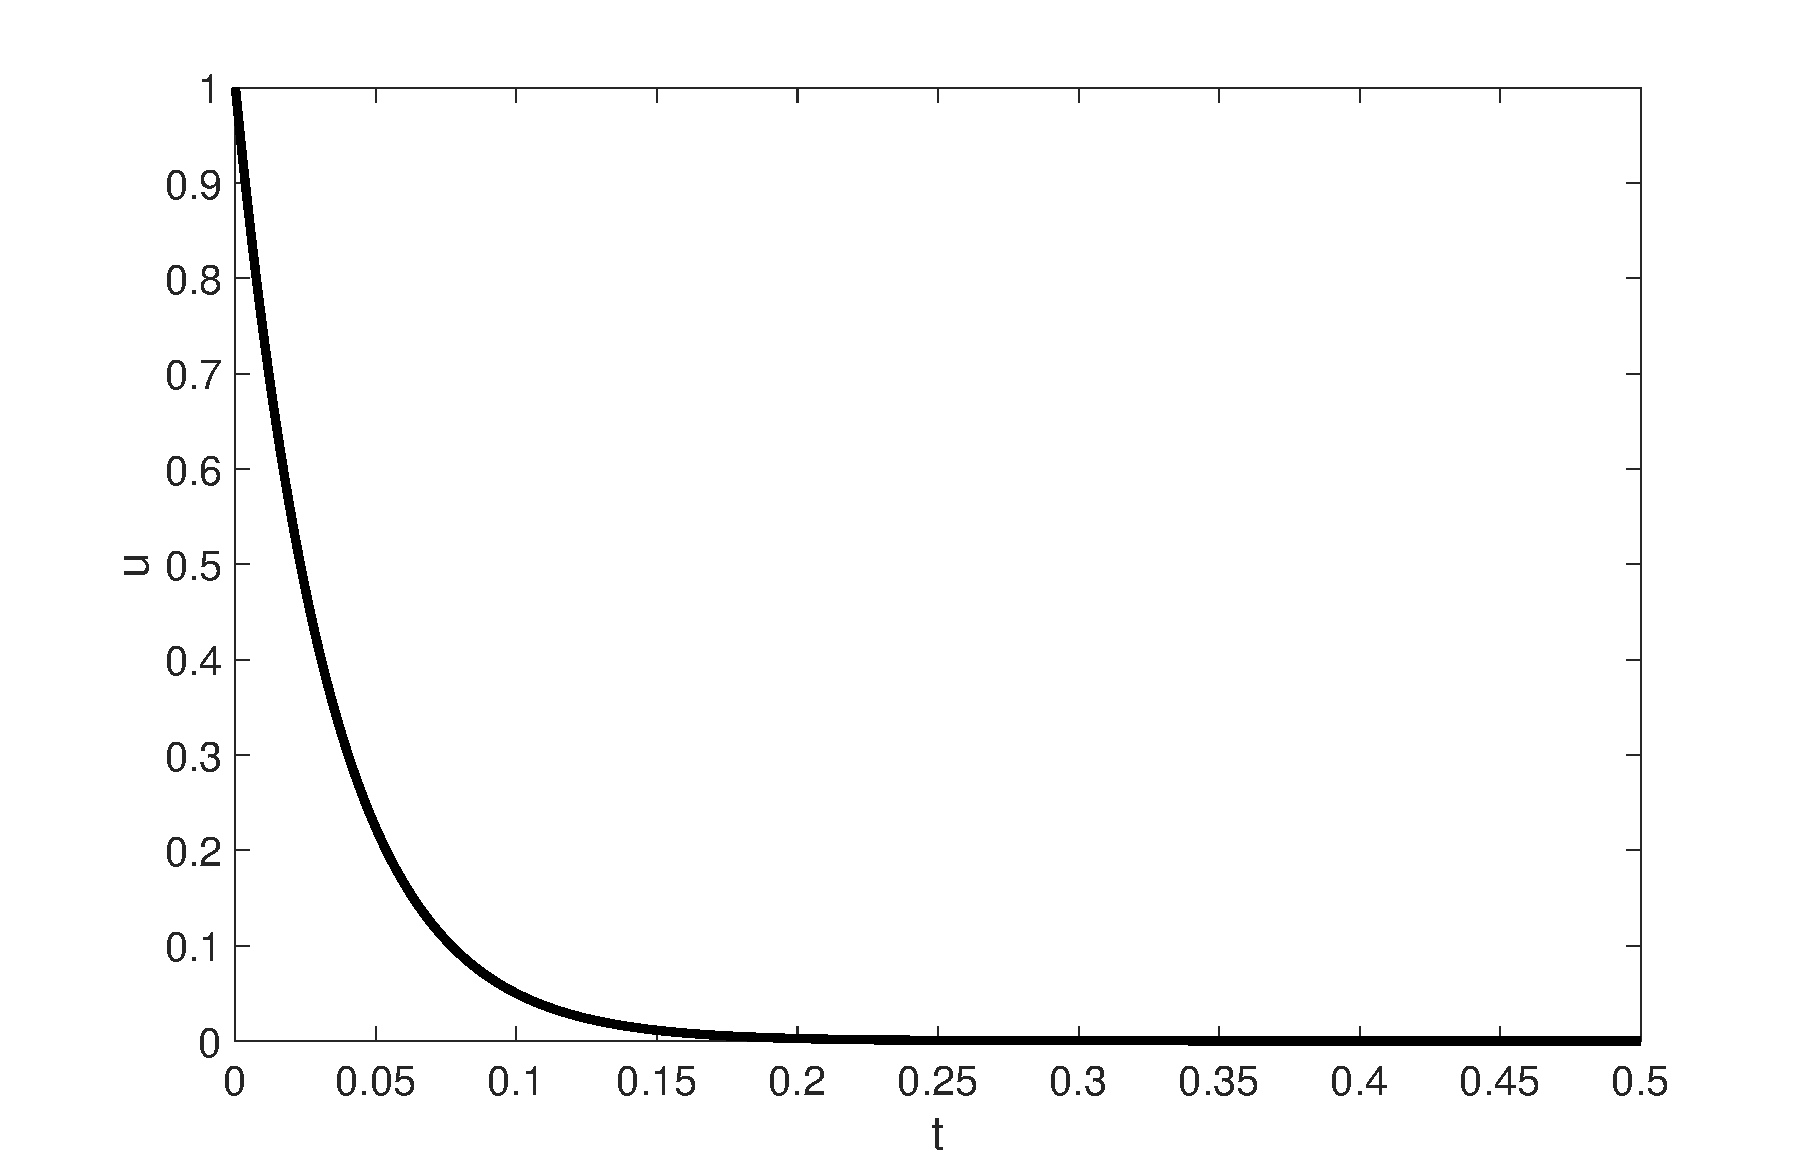
\includegraphics[height=4cm]{./figs/dahlquist_soln}
\end{equation*}
\end{itemize}
\end{frame}

%%%%%%%%%%%%%%%%%%%%%%%%%%%%%%%%%%%%%%%%%%%%

\begin{frame}{Euler's method approximation}
\begin{itemize}
    \item Euler's method for the model problem:
    \[
    u_{i+1} = u_i + h(\lambda u_i) = (1 + h \lambda) u_i, \qquad i = 0,1,2, \ldots
    \]
    
    \item Choose $\lambda = -30, u_0 =1, h = 0.1$
    \cols{    
    \begin{center}
        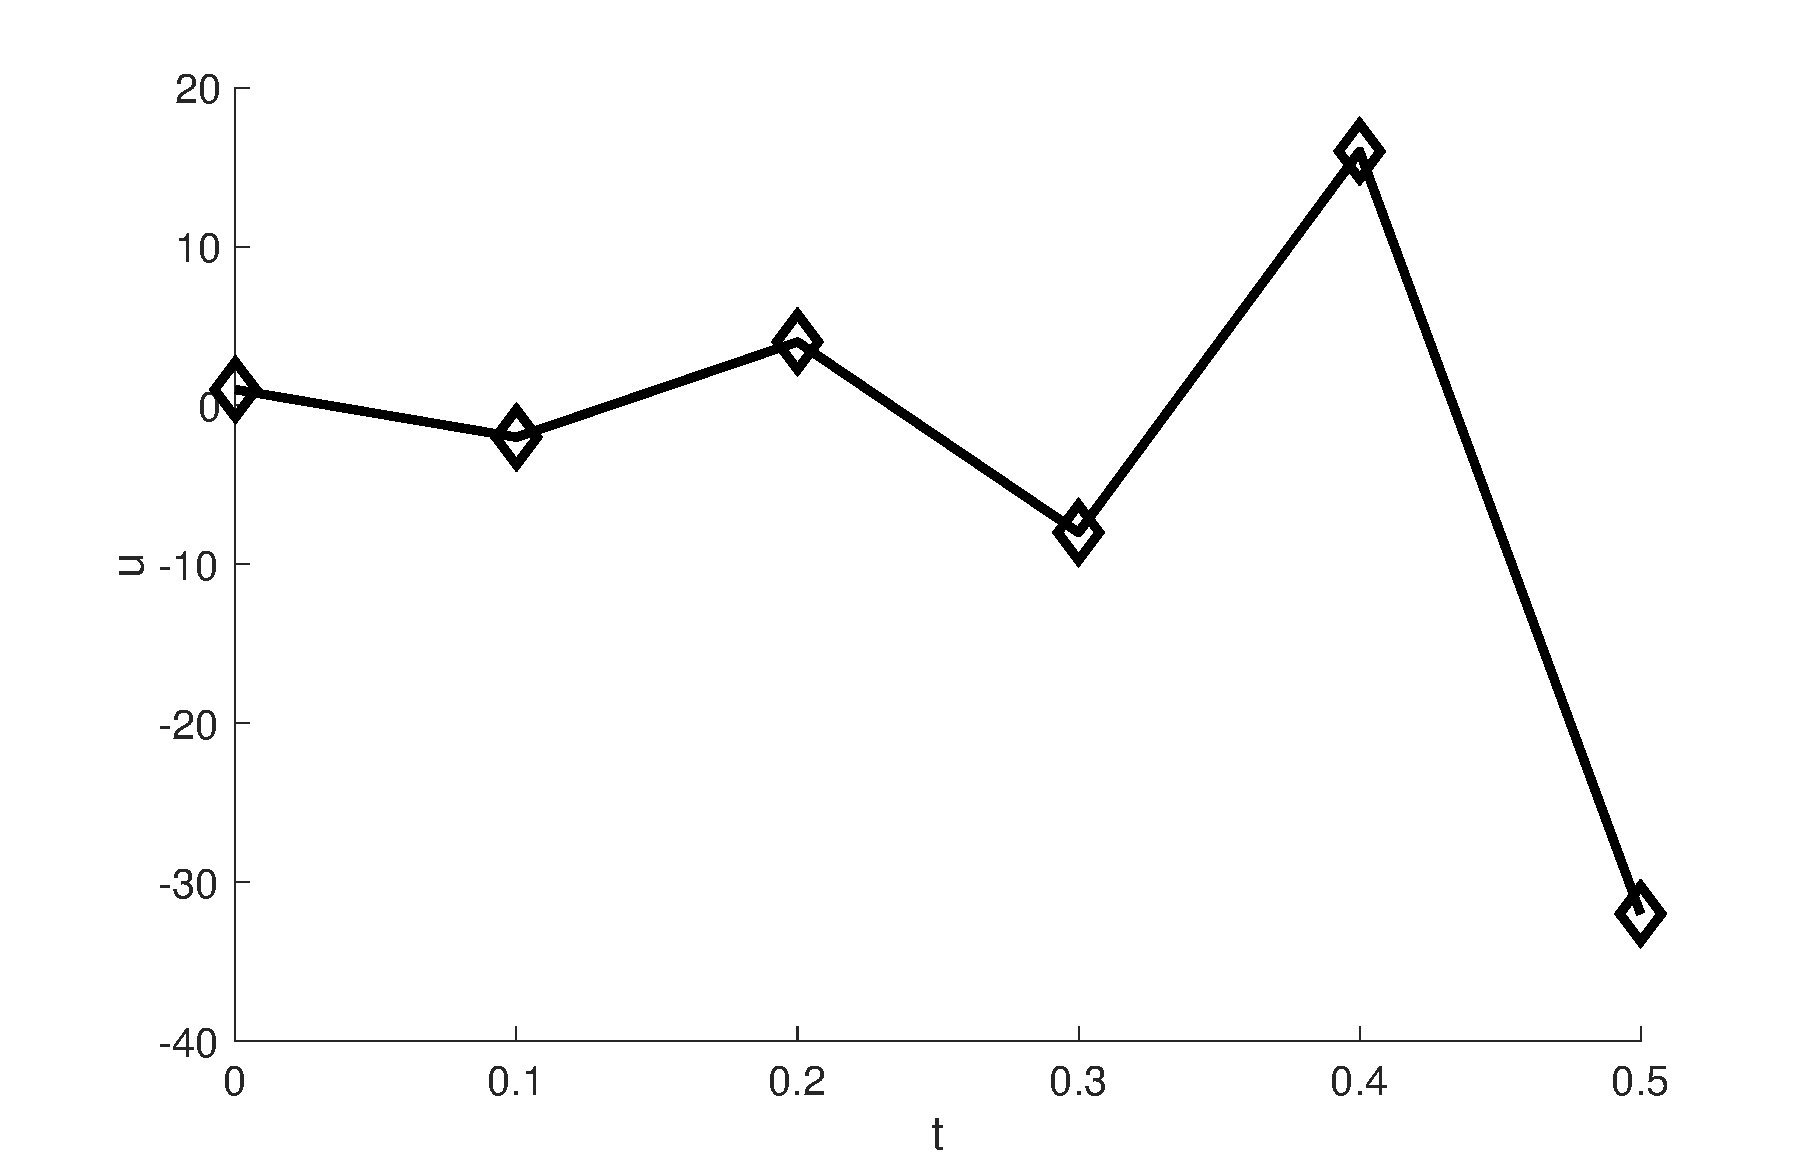
\includegraphics[height=4cm]{./figs/dahlquist_euler_soln}
    Euler solution
    \end{center}
    }{
    \begin{center}
        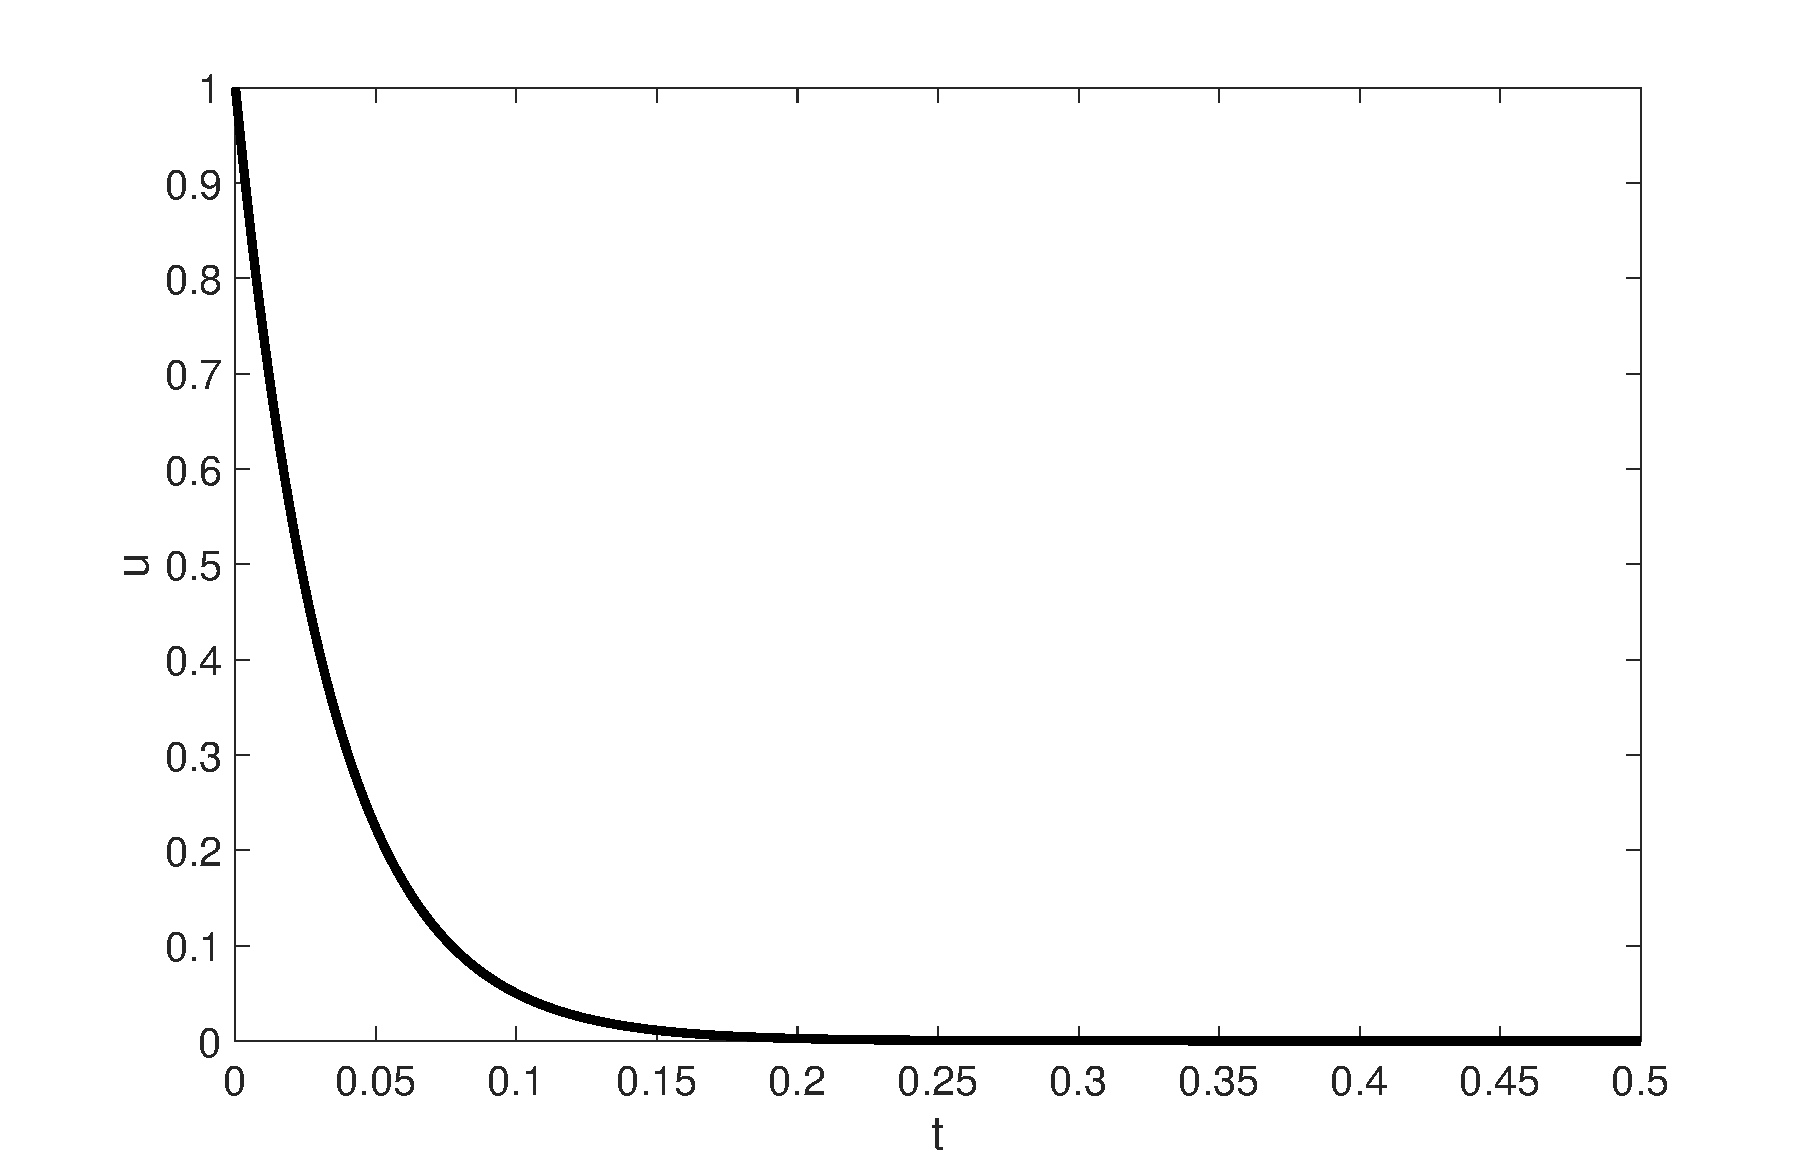
\includegraphics[height=4cm]{./figs/dahlquist_soln}
    True solution
    \end{center}
    }

    \item This is \textbf{numerical instability}

\end{itemize}
\end{frame}

%%%%%%%%%%%%%%%%%%%%%%%%%%%%%%%%%%%%%%%%%%%%

\begin{frame}{What went wrong?}
    \cols{    
    \begin{center}
        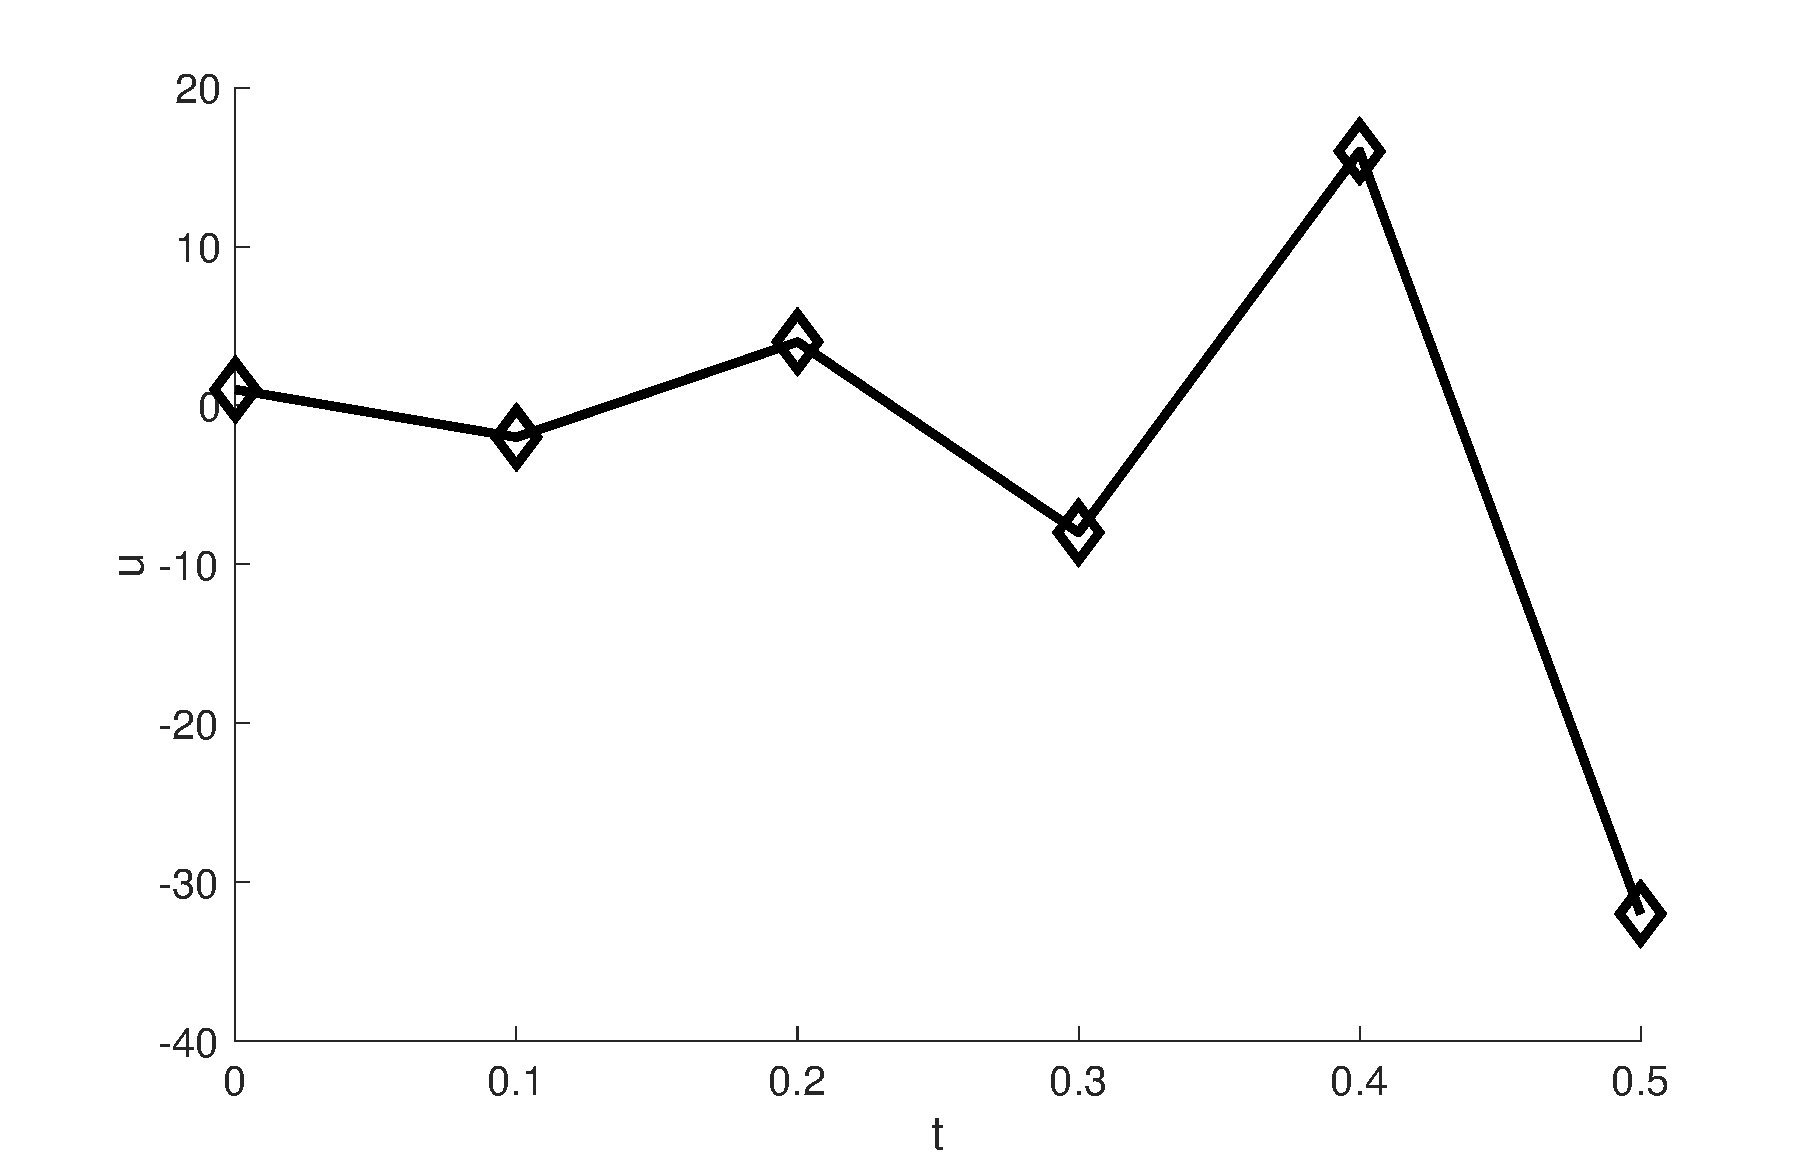
\includegraphics[height=4cm]{./figs/dahlquist_euler_soln}
    Euler solution
    \end{center}
    }{
    \begin{center}
        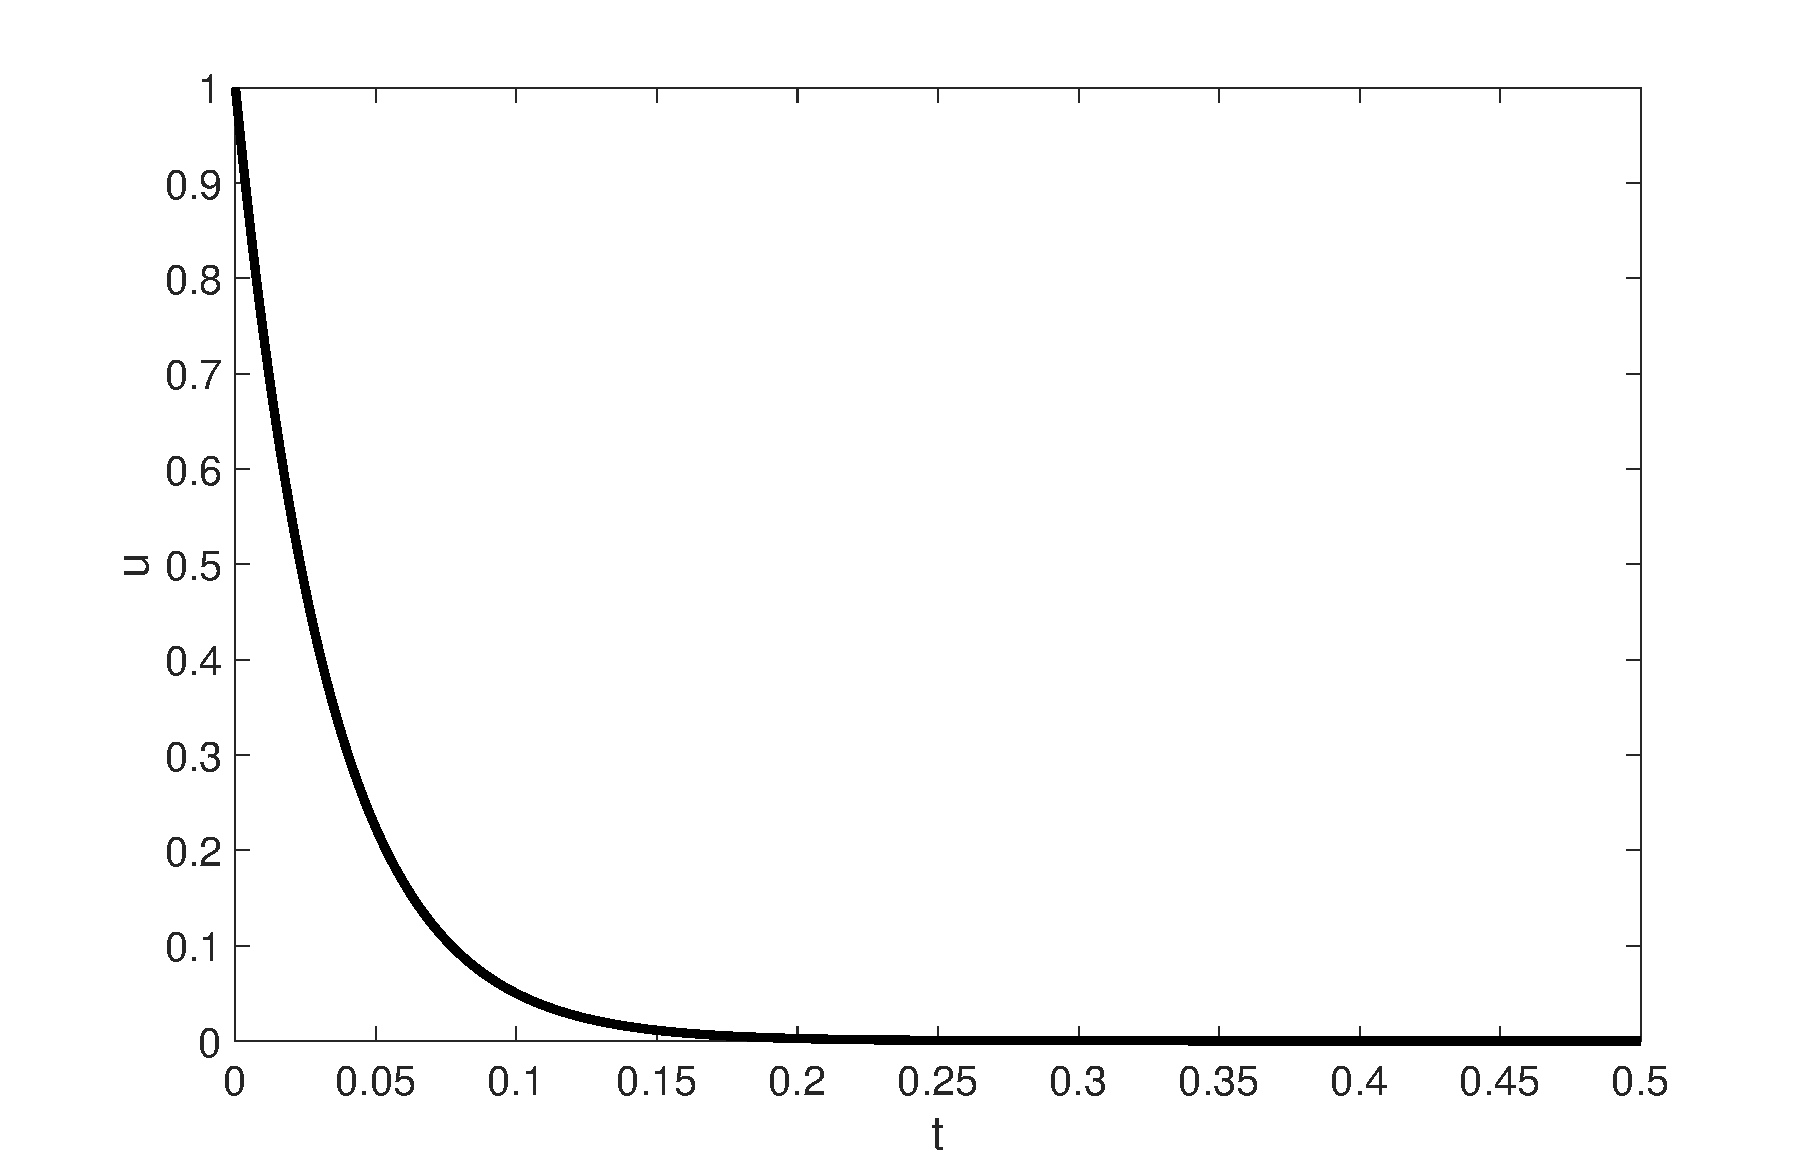
\includegraphics[height=4cm]{./figs/dahlquist_soln}
    True solution
    \end{center}
    }
\vspace{6mm}
What went wrong?
\begin{itemize}
    \item Didn't choose $h$ small enough
    \item The amplification factor is $1-30(0.1)=-2$ 
    \item Numerical solution is growing (!?) 
\end{itemize}
\end{frame}	

%%%%%%%%%%%%%%%%%%%%%%%%%%%%%%%%%%%%%%%%%%%%

\begin{frame}{Amplification factor}

\begin{alertblock}{Question}
    Why did the numerical solution grow?
\end{alertblock}

\begin{itemize}
    \item Euler's method is $u_{i+1} = u_i + h f(u_i)$ for $u' = \lambda u$ yields
    \begin{align*}
        u_{i+1} &= u_i + h \lambda u_i \\
                &= u_i( 1 + h\lambda) \\ 
        \implies |u_{i+1}| &= |1+h\lambda| |u_i| 
    \end{align*}



   \item Or more intuitively, 
   $$
        \underbrace{|u_{i+1}|}_{\text{new}} = \underbrace{|1+h\lambda|}_{\text{amplification factor}} \underbrace{|u_i|}_{\text{old}} 
   $$
   \item For decay we need  
        $$ |1+h\lambda| < 1$$

\end{itemize}

\end{frame}	

%%%%%%%%%%%%%%%%%%%%%%%%%%%%%%%%%%%%%%%%%
\begin{frame}{Stability Region}
\begin{itemize}
    \item Apply a Runge--Kutta method to $u'=\lambda u$:
    \[u_{i+1}=R(z)u_i,\qquad z=h\lambda.\]
    \item $R(z)$ is the method's amplification factor.
\end{itemize}
\define{Stability Region}{The region of absolute stability is
\[\{z\in\mathbb{C}: |R(z)|\leq1\}.\]
Inside the region where $|R(z)|<1$, the numerical solution decays.}
\keyidea{Choose $h$ so that $h\lambda$ lies in the stability region. Accuracy and computational cost also matter.}
% Boundary points can remain bounded without reproducing physical decay.
\end{frame}

\begin{frame}{Visualizing Stability Regions}

    \begin{center}
        \includegraphics[scale=0.4]{figs/rk_stability.png}
    \end{center}
    \begin{itemize}
        \item Stability regions are visualized in the complex plane
        \item The small blue circle is the stability region for Euler's method
        \item The largest magenta region is for RK4
    \end{itemize}
    
\end{frame}

%%%%%%%%%%%%%%%%%%%%%%%%%%%%%%%%%%%%%%%%%

\begin{frame}{Choosing a stable $h$}

\begin{example}
What value of $h$ would give a stable solution for Euler's method for the IVP
    \begin{align*}
    u^{'}(t) &= -30 u(t), \qquad  t \in [0,0.5]\\
    u(0) &= 1
    \end{align*}   

\end{example}
\begin{itemize}
    \item Euler's method yields 
        \begin{align*}
            u_{i+1} &= u_i  -30 h u_i \\ 
                    &= u_i(1 -30 h ) \\ 
            \implies |u_{i+1}| &= |1-30h| |u_i| 
        \end{align*}
    \item For decay we need $|1-30h| < 1$ or 
        \begin{align*}
            -1 &< 1-30h < 1\\
            -2 &< -30h < 0\\ 
             1/15 > h > 0
        \end{align*}
    \item Choose $0<h<1/15$. At $h=1/15$, the solution oscillates without decay.

\end{itemize}
\end{frame}	

% %%%%%%%%%%%%%%%%%%%%%%%%%%%%%%%%%%%%%%%%%%%%
\sectionframe{The Pendulum}
% %%%%%%%%%%%%%%%%%%%%%%%%%%%%%%%%%%%%%%%%%%%%

\begin{frame}{Physical Setup}

\begin{figure}[H]
    \centering
    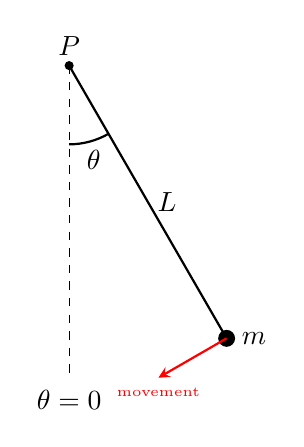
\begin{tikzpicture}[>=stealth]
    \def\L{4}        % Length of the pendulum
    \def\ang{30}     % Angle from vertical
    \draw[thick] (0,0) -- ({\L*sin(\ang)},{-\L*cos(\ang)});
    \draw[fill] (0,0) circle (0.05) node[above] {$P$};
    \draw[fill] ({\L*sin(\ang)},{-\L*cos(\ang)}) circle (0.1) node[right=2pt] {$m$};
    \draw[->,red,thick] ({\L*sin(\ang)},{-\L*cos(\ang)}) -- ++({-cos(\ang)*1.0},{-sin(\ang)*1.0}) node [below] {\tiny movement};
    \draw[thick] (0,-1) arc[start angle=-90, end angle={-90+\ang}, radius=1];
    \node at (0.1,-1.2) [right] {$\theta$};
    \draw[dashed] (0,0) -- (0,-{\L}) node [below] {$\theta=0$};
    \node at ({\L*sin(\ang)/2},{-\L*cos(\ang)/2}) [right] {$L$};
    \end{tikzpicture}
    \label{fig:pend}
\end{figure}
\begin{itemize}
    \item Pendulum of length $L$ is attached to a bob of mass $m$
    \item Pendulum may pivot about point $P$, i.e. it can oscillate
    \item Motion is described by the angular displacement  $\theta(t)$ 
    \item The neutral hanging position is $\theta=0$
\end{itemize}

\end{frame}

% -------------

\begin{frame}{Objective}

\textbf{Variables: }
\begin{itemize}
    \item $t$ = time 
    \item $\theta(t)$ = angular displacement of the pendulum at time $t$
    \item $L$ = length of the rod 
    \item $m$ = mass of the weight 
    \item $\omega=\theta'$ = angular velocity
\end{itemize}

\vspace{1cm}
\begin{block}{Goal}
Derive a differential equation describing the motion of the pendulum using the variables above.
\end{block}
\end{frame}

% ------------------
\begin{frame}{Initial Conditions}
\begin{figure}[H]
    \centering
    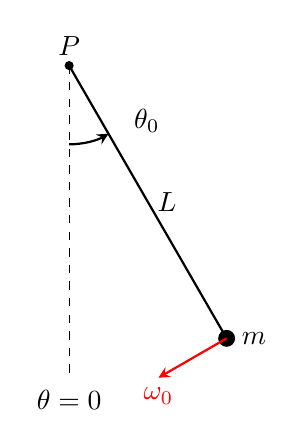
\begin{tikzpicture}[>=stealth]
    \def\L{4}        % Length of the pendulum
    \def\ang{30}     % Angle from vertical
    \draw[thick] (0,0) -- ({\L*sin(\ang)},{-\L*cos(\ang)});
    \draw[fill] (0,0) circle (0.05) node[above] {$P$};
    \draw[fill] ({\L*sin(\ang)},{-\L*cos(\ang)}) circle (0.1) node[right=2pt] {$m$};
    \draw[->,red,thick] ({\L*sin(\ang)},{-\L*cos(\ang)}) -- ++({-cos(\ang)*1.0},{-sin(\ang)*1.0}) node [below] {$\omega_0$};
    \draw[thick,->] (0,-1) arc[start angle=-90, end angle={-90+\ang}, radius=1];
    \node at (0.7,-0.7) [right] {$\theta_0$};
    \draw[dashed] (0,0) -- (0,-{\L}) node [below] {$\theta=0$};
    \node at ({\L*sin(\ang)/2},{-\L*cos(\ang)/2}) [right] {$L$};
    \end{tikzpicture}
\end{figure}

\begin{itemize}
    \item Initial position $\theta(0)=\theta_0$
    \item Initial angular velocity $\theta'(0) = \omega_0$
\end{itemize}
\begin{center}
    \textit{We pull the bob to the right, and then give it a tap in the left direction.}
\end{center}
    
\end{frame}

% ------------------

\begin{frame}{Free Body Diagram}
\begin{columns}[c]
% ================= LEFT COLUMN =================
\begin{column}{0.35\textwidth}
Three forces
\begin{itemize}
    \item Tension 
    \item Friction 
    \item Weight
\end{itemize}
\vspace{1cm}
Tangential forces change the angular velocity. The radial resultant supplies centripetal acceleration. 

\end{column}

% ================= RIGHT COLUMN =================
\begin{column}{0.50\textwidth}
\begin{figure}
    \centering
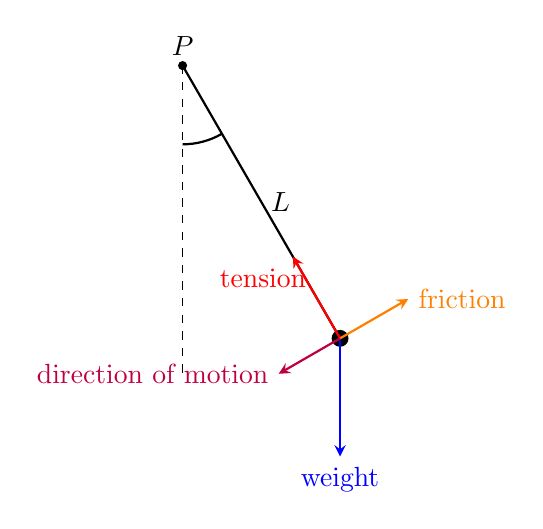
\begin{tikzpicture}[>=stealth,scale=1]
    \def\L{4}
    \def\ang{30}

    % Coordinates
    \coordinate (P) at (0,0);
    \coordinate (M) at ({\L*sin(\ang)},{-\L*cos(\ang)});

    % Rod and pivot
    \draw[thick] (P) -- (M);
    \draw[fill] (P) circle (0.05) node[above] {$P$};
    \draw[fill] (M) circle (0.10);

    % Dashed vertical (theta=0 reference)
    \draw[dashed] (P) -- (0,-\L);
    % \node at (0,-\L) [below] {$\theta = 0$};

    % Angle arc
    \draw[thick] (0,-1) arc[start angle=-90, end angle={-90+\ang}, radius=1];
    % \node at (0.9,-0.5) {$\theta$};

    % Forces
    % Gravity
    \draw[->,thick,blue] (M) -- ++(0,-1.5) node[below] {weight};

    % Tension
    \draw[->,thick,red] (M) -- ({0.7*\L*sin(\ang)},{-0.7*\L*cos(\ang)})
        node[midway,above left] {tension};

    % friction 
    \draw[->,thick,orange] (M) --
        ++({cos(\ang)}, {sin(\ang)}) node[right] {friction};

    % tangent 
    \draw[->,thick,purple] (M) --
        ++({-0.9*cos(\ang)},{-0.9*sin(\ang)})
        node[left] {direction of motion};


    % Label length
    \node at ({\L*sin(\ang)/2},{-\L*cos(\ang)/2}) [right] {$L$};
\end{tikzpicture}
\end{figure}
\end{column}
\end{columns}
\end{frame}



% --------------------------

\begin{frame}{Tangential vs. Radial}
\begin{columns}[c]
% ================= LEFT COLUMN =================
\begin{column}{0.35\textwidth}
\begin{itemize}
    \item Resolve weight into tangential and radial components 
    \item Radially, $T-mg\cos\theta=mL\omega^2$, where $\omega=\theta'$
    \item Tangential component of the weight 
    $W_t = -mg \sin \theta$
    \item Model tangential damping as $F_d=-c\,\theta'$, $c\ge0$
\end{itemize}


\end{column}

% ================= RIGHT COLUMN =================
\begin{column}{0.50\textwidth}
\begin{figure}
    \centering
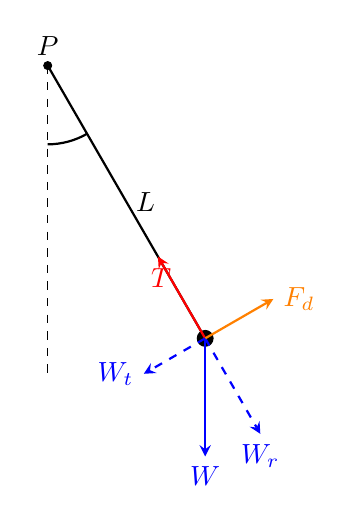
\begin{tikzpicture}[>=stealth,scale=1]
    \def\L{4}
    \def\ang{30}

    % Coordinates
    \coordinate (P) at (0,0);
    \coordinate (M) at ({\L*sin(\ang)},{-\L*cos(\ang)});

    % Rod and pivot
    \draw[thick] (P) -- (M);
    \draw[fill] (P) circle (0.05) node[above] {$P$};
    \draw[fill] (M) circle (0.10);

    % Dashed vertical (theta=0 reference)
    \draw[dashed] (P) -- (0,-\L);
    % \node at (0,-\L) [below] {$\theta = 0$};

    % Angle arc
    \draw[thick] (0,-1) arc[start angle=-90, end angle={-90+\ang}, radius=1];
    % \node at (0.9,-0.5) {$\theta$};

    % Forces
    % Gravity
    \draw[->,thick,blue] (M) -- ++(0,-1.5) node[below] {$W$};
    \draw[->,thick,dashed,blue] (M) -- ({1.35*\L*sin(\ang)},{-1.35*\L*cos(\ang)}) node[below] {$W_r$};

    % Tension
    \draw[->,thick,red] (M) -- ({0.7*\L*sin(\ang)},{-0.7*\L*cos(\ang)})
        node[midway,above left] {$T$};

    % friction 
    \draw[->,thick,orange] (M) --
        ++({cos(\ang)}, {sin(\ang)}) node[right] {$F_d$};

    % tangent 
    \draw[->,thick,blue,dashed] (M) --
        ++({-0.9*cos(\ang)},{-0.9*sin(\ang)})
        node[left] {$W_t$};

    % Label length
    \node at ({\L*sin(\ang)/2},{-\L*cos(\ang)/2}) [right] {$L$};
\end{tikzpicture}
\end{figure}
\end{column}
\end{columns}
\end{frame}


% --------------------------


\begin{frame}{Derivation}
    
\textbf{Step 1. Coordinates and Kinematics}

Take two derivatives of the Arc length formula $s = L\theta$  
:
\[
s''  = L\theta''=a.
\]

\vspace{3mm}

\textbf{Step 2. Newton's Law}

Newton's Second Law says the tangential forces satisfy 
$$ \sum F = ma=mL\theta''$$

\vspace{3mm}

\textbf{Step 3. Sum of Forces}
The two forces are tangential component of weight and friction
\[ 
\sum F = W_{\text{t}} +F_d = -mg \sin\theta - c\,\theta'
\]


\vspace{3mm}

\textbf{Step 4. Putting it all together}
\begin{align*}
&-mg \sin\theta - c\,\theta'=mL\,\theta''\\
&\boxed{mL\,\theta'' + c\,\theta'  +mg \sin\theta=0}
\end{align*}
\end{frame}

%%%%%%%%%%%%%%%%%%%%%%%%%%%%%%%%%%%%%%%%%%%%

\begin{frame}{Types of Initial Conditions}

\begin{block}{Equation for the Pendulum}
\[
mL\,\theta'' + c\,\theta'  +mg \sin\theta=0
\]
we must specify \emph{two} initial conditions.
\end{block}

\vspace{2mm}


\vspace{3mm}

\textbf{Common choices of initial conditions:}

\begin{itemize}
    \item \textbf{Released from rest:}  
    \[
      \theta(0)=\theta_0, \qquad \theta'(0)=0.
    \]

    \item \textbf{Given an initial push:}  
    \[
      \theta(0)=\theta_0, \qquad \theta'(0)=\omega_0.
    \]

    \item \textbf{Starting at the bottom with a kick:}  
    \[
      \theta(0)=0, \qquad \theta'(0)=\omega_0.
    \]

    \item \textbf{Starting near the top (unstable):}  
    \[
      \theta(0)\approx \pi, \qquad \theta'(0)\approx 0.
    \]
\end{itemize}

\end{frame}

% Damping convention: c multiplies angular velocity in a tangential FORCE;
% a torque damping coefficient would instead accompany m L^2.
\begin{frame}{The Pendulum as a First-Order System}
Set $y_1=\theta$ and $y_2=\theta'$:
\[
\begin{cases}
y_1'=y_2,\\
y_2'=-\dfrac{c}{mL}y_2-\dfrac{g}{L}\sin y_1,
\end{cases}
\qquad
\begin{cases}
y_1(0)=\theta_0,\\
y_2(0)=\omega_0.
\end{cases}
\]
\keyidea{Apply Euler, RK4, or an adaptive ODE solver to this two-component system.}
\end{frame}

\begin{frame}{Visualizing the Solution}
\begin{itemize}
    \item We can solve $mL\,\theta'' + c\,\theta'  +mg \sin\theta=0$ with Euler's method and plot
    \begin{figure}
        \centering
        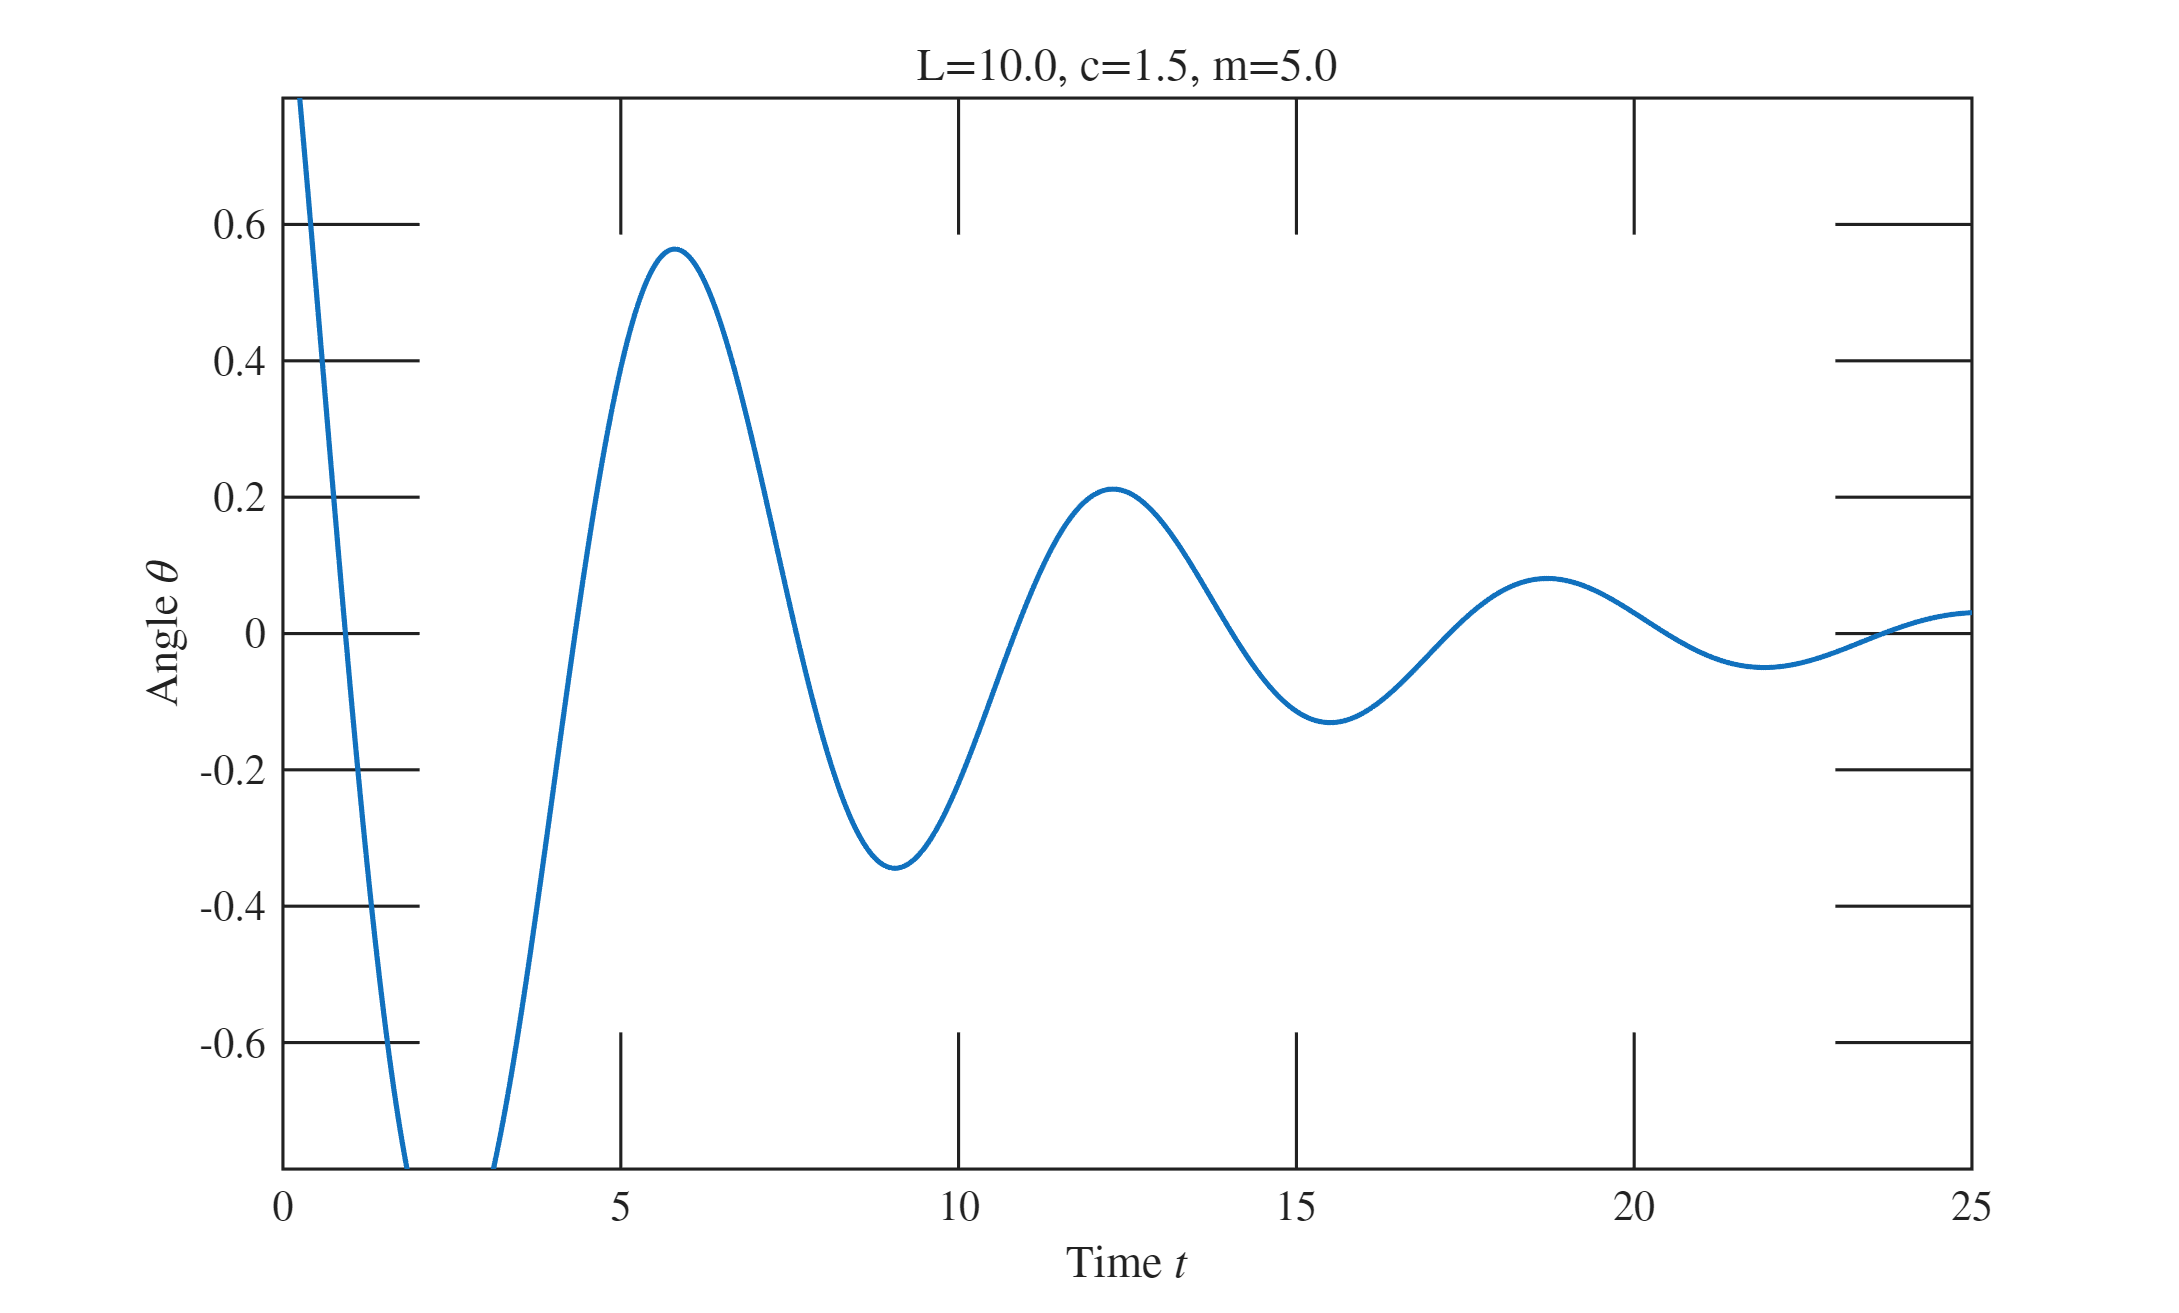
\includegraphics[width=0.9\linewidth]{figs/pend.png}
    \end{figure}
    \item<2> But that's boring
\end{itemize}
\end{frame}

% %%%%%%%%%%%%%%%%%%%%%%%%%%%%%%%%%%%%%%%%%%%%
\begin{frame}[fragile]{Making Animations}
\begin{itemize}
    \item An \textbf{animation} is made by plotting the pendulum in increments of time $\Delta t$ and writing it as a frame of a video
    \item First, solve $mL\,\theta'' + c\,\theta'  +mg \sin\theta=0$
    \item Plot pendulum at $t=0$, save it. 
    \item Plot pendulum at $t=t_1$, save it. 
    \item Keep going up to $t=t_n$.
\end{itemize}
\begin{lstlisting}[mathescape]
% Pseudocode: solve the system, then draw each state
[t,u] = solve_pendulum()
for i = 1 : n
    plot(state of pendulum at time $t_i$)
    imwrite(plot_to_gif)
end
\end{lstlisting}
\end{frame}


% -----------
% \begin{frame}{Released from Rest}
% \centering

% \movie[
%   autostart,
%   loop,
%   width=0.6\linewidth,
%   height=0.6\linewidth
% ]{%
%   \parbox[c][0.6\linewidth][c]{0.6\linewidth}{%
%     \centering
%     \fbox{%
%       \parbox[c][0.4\linewidth][c]{0.5\linewidth}{%
%          \large\textbf{Click to play}
%       }
%     }
%   }
% }{figs/pendulum1.mp4}
% \end{frame}
% % -----------
% \begin{frame}{Initial Kick}
% \centering

% \movie[
%   autostart,
%   loop,
%   width=0.6\linewidth,
%   height=0.6\linewidth
% ]{%
%   \parbox[c][0.6\linewidth][c]{0.6\linewidth}{%
%     \centering
%     \fbox{%
%       \parbox[c][0.4\linewidth][c]{0.5\linewidth}{%
%          \large\textbf{Click to play}
%       }
%     }
%   }
% }{figs/pendulum2.mp4}
% \end{frame}
% % -----------
% \begin{frame}{Kick from Neutral Position}
% \centering

% \movie[
%   autostart,
%   loop,
%   width=0.6\linewidth,
%   height=0.6\linewidth
% ]{%
%   \parbox[c][0.6\linewidth][c]{0.6\linewidth}{%
%     \centering
%     \fbox{%
%       \parbox[c][0.4\linewidth][c]{0.5\linewidth}{%
%          \large\textbf{Click to play}
%       }
%     }
%   }
% }{figs/pendulum3.mp4}
% \end{frame}
% % -----------
% \begin{frame}{Almost 180 Start}
% \centering

% \movie[
%   autostart,
%   loop,
%   width=0.6\linewidth,
%   height=0.6\linewidth
% ]{%
%   \parbox[c][0.6\linewidth][c]{0.6\linewidth}{%
%     \centering
%     \fbox{%
%       \parbox[c][0.4\linewidth][c]{0.5\linewidth}{%
%          \large\textbf{Click to play}
%       }
%     }
%   }
% }{figs/pendulum4.mp4}
% \end{frame}
% -----------


% %%%%%%%%%%%%%%%%%%%%%%%%%%%%%%%%%%%%%%%%%%%%
% \sectionframe{Visualizing Stability of a Method}
% %%%%%%%%%%%%%%%%%%%%%%%%%%%%%%%%%%%%%%%%%%%%


% \begin{frame}{Region of Stability}

% \begin{block}{Test Problem} 
% For this test IVP, let \(\lambda \in \mathbb{C}\):
% \[
% \begin{cases}
% u^{\prime}(t) = \lambda u(t), \quad t \in [0, T], \\
% u(0) = u_0.
% \end{cases}
% \]
% \(\lambda\) often represents an \textit{eigenvalue} of the system, scaling the rate of change.
% \end{block}

% \define{Stability Region}{

% The \textbf{region of stability} for a time-stepping method is the set of \(z = \lambda h\) in the complex plane for which the numerical solution for the test problem remains bounded:
% \[
% |G(z)| \leq 1,
% \]
% where \(G(z)\) is the method's amplification factor.
% }

% \end{frame}

% %%%%%%%%%%%%%%%%%%%%%%%%%%%%%%%%%%%%%%%%%%%%

% \begin{frame}{Stability Region of Euler's Method}

% \begin{itemize}
%     \item For Euler’s method the amplification factor is:
%     \[
%     G(z) = 1 + \lambda h = 1 + z.
%     \]

%     \item Stability condition is
%     \[
%     |G(z)| = |1 + z| \leq 1.
%     \]

%     \item The stability region is the set:
%     \[
%     S = \{ z \in \mathbb{C} \;|\; |1 + z| \leq 1 \}.
%     \]
%     This is a disk of radius 1 centered at \(-1\) in the complex plane.
% \end{itemize}

% \end{frame}

% %%%%%%%%%%%%%%%%%%%%%%%%%%%%%%%%%%%%%%%%%%%%

% \begin{frame}{Visualizing the Stability Region for Euler's Method}

% \begin{itemize}
%     \item The stability region is a circle of radius 1 centered at \(z_0 = -1\).
%     \item Points inside this circle correspond to stable step-size and eigenvalue combinations.
% \end{itemize}

% \begin{center}
% \begin{tikzpicture}[scale=1.2]
%     % Stability region (circle)
%     \draw[fill=gray!30] (-1,0) circle (1);
%     % Axes
%     \draw[->, thick] (-3,0)--(1,0) node[right] {\(\mathrm{Re}(h\lambda)\)};
%     \draw[->, thick] (0,-1.5)--(0,1.5) node[above] {\(\mathrm{Im}(h\lambda)\)};
%     % Labels
%     \node at (-1, 0) {\(\bullet\)};
%     \node[below] at (-1,0) {\(-1\)};
%     \node[right] at (0,1) {\(i\)};
%     \node[right] at (0,-1) {\(-i\)};
%     % Boundary
%     \draw[dashed] (-1,-1) -- (-1,1);
%     \draw[dashed] (0,1) -- (0,-1);
% \end{tikzpicture}
% \end{center}
% \begin{block}{Idea}
%     Plot shows us the poolsize of stable $h$ values for Euler's.
% \end{block}
% \end{frame}

% %%%%%%%%%%%%%%%%%%%%%%%%%%%%%%%%%%%%%%%%%%%%

% \begin{frame}{Region of Stability for RK2b}

% \begin{itemize}
%     \item For the model problem \( u^\prime = \lambda u \), RK2b gives:
%     \begin{align*}
%         K_1 &= \lambda u_j, \\
%         K_2 &= \lambda \left(u_j + \frac{h}{2}\lambda u_j\right), \\
%         u_{j+1} &= u_j \left(1 + h \lambda + \frac{1}{2} (h \lambda)^2\right).
%     \end{align*}

%     \item Amplification Factor:
%     \[
%     G(z) = \left| \frac{u_{j+1}}{u_j} \right| = \left|1 + z + \frac{1}{2}z^2 \right|, \quad z = h \lambda.
%     \]

%     \item Stability Condition:
%     Want all \( z \in \mathbb{C} \) such that:
%     \[
%     \left|1+ z + \frac{1}{2}z^2\right| < 1.
%     \]


% \end{itemize}
% \end{frame}



% %%%%%%%%%%%%%%%%%%%%%%%%%%%%%%%%%%%%%%%%%%%%%%%%%%%%%%%%%%%%%%%%%%%%%%%%%
% \begin{frame}[fragile]
% \frametitle{Region of Stability for RK4}
% \begin{itemize}
	
%    \item After similar derivations as earlier we get
% 	\[
% 	G = \left |1 + (h \lambda) + \frac{1}{2}(h \lambda)^2 + \frac{1}{6}(h \lambda)^3 + \frac{1}{24}(\lambda h)^4 \right|
% 	\]
	
%    \item Stability Condition:
% 	\[
% 	G(z) = \left |1 + z + \frac{1}{2}z^2 + \frac{1}{6}z^3 + \frac{1}{24}z^4 \right| < 1
% 	\]
	
%    \item We can plot the stability region numerically 
% \end{itemize}

% \begin{tiny}
% \begin{lstlisting}[mathescape]
% [x,y] = meshgrid(linspace(-4,4), linspace(-4,4));
% z = x + 1i*y;
% contour(x,y,abs(1+z+(1/2)*z.^2+(1/6)*z.^3+(1/24)*z.^4),[1, 1]);
% \end{lstlisting}
% \end{tiny}


% \end{frame}

% \begin{frame}{Takeaway}

%     \begin{itemize}
%         \item Stability Regions gives us a way to visualize the pool size of good parameter choices for a time-stepping algorithm

        
%     \begin{center}
%         \includegraphics[scale=0.5]{figs/rk_stability.png}
%     \end{center}
    

%         \item larger the region $\implies$ more reliable the algorithm
    
    
%     \end{itemize}
    
% \end{frame}

%%%%%%%%%%%%%%%%%%%%%%%%%%%%%%%%%%%%%%%%%%%%%%%%%%%%%%%%%%%%%%%%%%%
\end{document}

